\documentclass[a4paper]{article}

\usepackage{forest}

\usepackage[english]{babel}
\usepackage[utf8]{inputenc}
\usepackage{graphicx}
\usepackage{enumitem}
\usepackage{blindtext}
\usepackage{amsmath}
\graphicspath{ {./images/} }

\def\changemargin#1#2{\list{}{\rightmargin#2\leftmargin#1}\item[]}
\let\endchangemargin=\endlist 

\title{CS2500 Homework 4}
\author{Evan Wilcox}
\setlength\parindent{0pt}
    
\date{Due March 12, 2019}
    
\begin{document}
    \maketitle

    \begin{enumerate}

        \item
        \textbf{6.1-6} \\

        \begin{tabular}{ c|c c c c c c c c c c }
            Index & 1 & 2 & 3 & 4 & 5 & 6 & 7 & 8 & 9 & 10 \\ \hline
            Value & 23 & 17 & 14 & 6 & 13 & 10 & 1 & 5 & 7 & 12 \\
        \end{tabular}

        No this array is not a max heap because the right child at the 9th index of 
        the node at the 4th index has a value greater than the 4th node.

        \vspace{3cm}

        \item
        \textbf{6.1-7} \\

        \begin{center}
            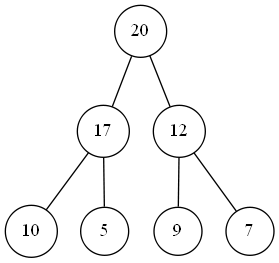
\includegraphics[scale=0.4]{61-7}

            \begin{tabular}{ c|c c c c c c c }
                Index & 1  & 2  & 3  & 4  & 5 & 6 & 7 \\ \hline
                Node  & 20 & 17 & 12 & 10 & 5 & 9 & 7 \\
            \end{tabular}
        \end{center}

        This is a 7 element tree and there are 4 leafs. \\
        The first leaf is at index $\lfloor n/2 \rfloor + 1 = 4$ \\ 
        The second leaf is at index $\lfloor n/2 \rfloor + 2 = 5$ \\
        The third leaf is at index $\lfloor n/2 \rfloor + 3 = 6$ \\
        The fourth leaf is at index $\lfloor n/2 \rfloor + 4 = 7$

        \newpage
        \item
        \textbf{6.2-1} \\

        \begin{center}
            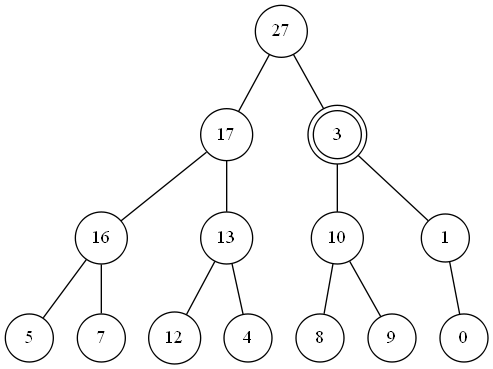
\includegraphics[scale=0.3]{62-1a} 
            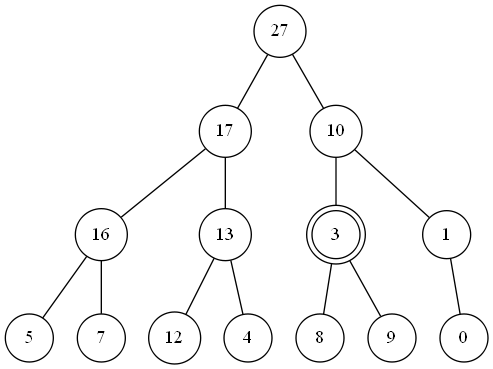
\includegraphics[scale=0.3]{62-1b} 
        \end{center}
        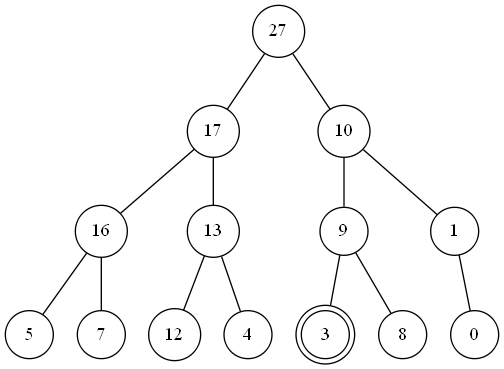
\includegraphics[scale=0.3]{62-1c}


        \item
        \textbf{6.2-3} \\
        Calling MAX-HEAPIFY$(A, i)$ when the element $A[i]$ is larger than its 
        children has no effect because that node is already a max heap. \\

        \item 
        \textbf{6.3-1} \\
        \begin{center}
            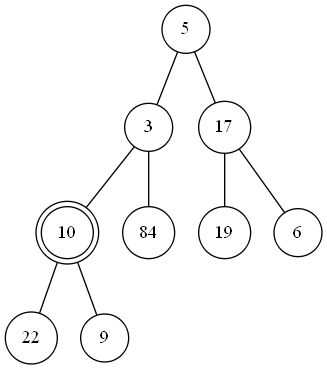
\includegraphics[scale=0.3]{63-1a} \phantom{hello}
            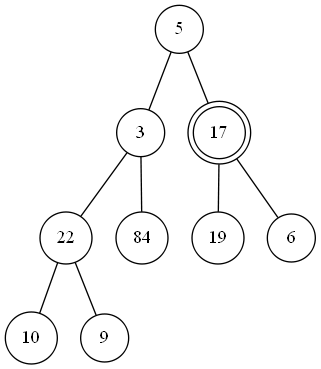
\includegraphics[scale=0.3]{63-1b} 
        \end{center}

        \begin{center}
            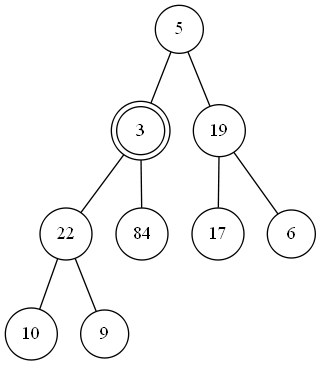
\includegraphics[scale=0.3]{63-1c} \phantom{hello}
            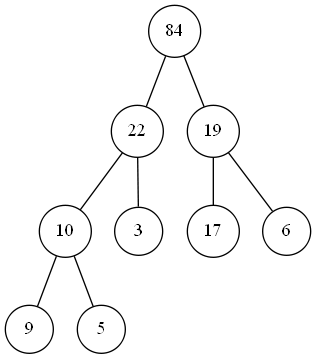
\includegraphics[scale=0.3]{63-1d} 
        \end{center}


        \item 
        \textbf{6.4-1} \\

        \begin{changemargin}{-1cm}{-1cm}
            \begin{center}
                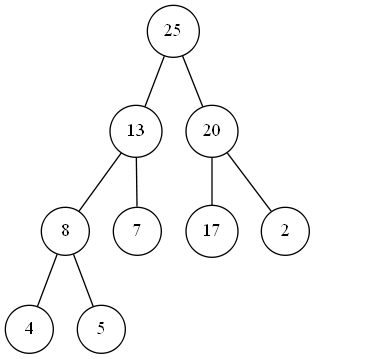
\includegraphics[scale=0.3]{64-1a} \phantom{space}
                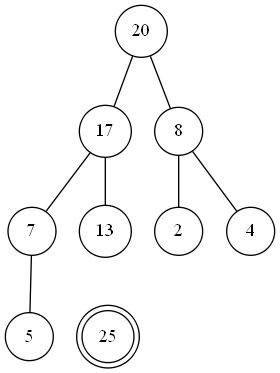
\includegraphics[scale=0.3]{64-1b} \phantom{space}
                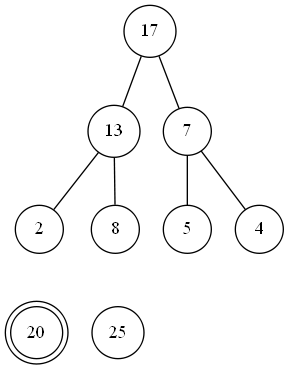
\includegraphics[scale=0.3]{64-1c} 
            \end{center}
            \vspace{0.5cm}
            \begin{center}
                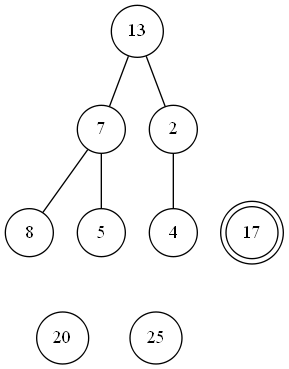
\includegraphics[scale=0.3]{64-1d} \phantom{space}
                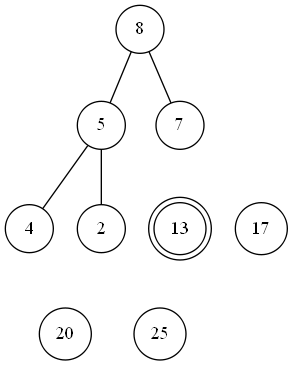
\includegraphics[scale=0.3]{64-1e} \phantom{space}
                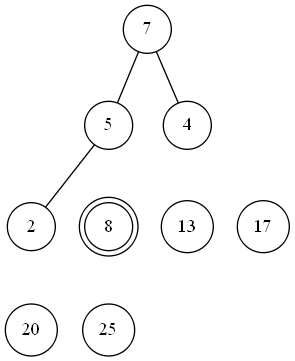
\includegraphics[scale=0.3]{64-1f}
            \end{center}
            \vspace{0.5cm}
            \begin{center}
                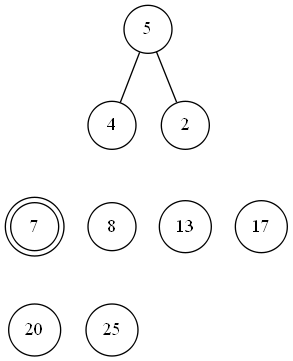
\includegraphics[scale=0.3]{64-1g} \phantom{space}
                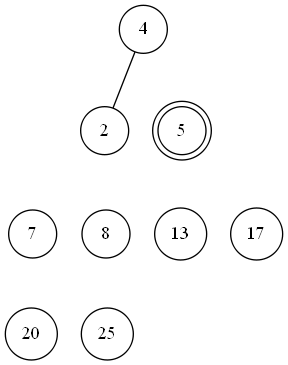
\includegraphics[scale=0.3]{64-1h} \phantom{space}
                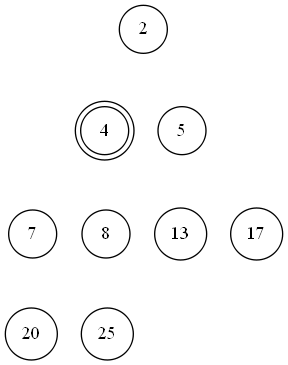
\includegraphics[scale=0.3]{64-1i} 
            \end{center}
        \end{changemargin}

        \begin{center}
            $A$
            \begin{tabular}{ |c|c|c|c|c|c|c|c|c| } \hline
                2 & 4 & 5 & 7 & 8 & 13 & 17 & 20 & 25 \\ \hline
            \end{tabular}
        \end{center}

        \newpage
        \item 
        \textbf{6.4-2} – show this invariant implemented as a c assert statement
        \begin{verbatim}
for(int j = 1; j <= i; j++)
{
    if(2 * j < heap-size)
    {    
        # left child
        assert(A[j] >= A[2 * j]);
    }
    
    if(2 * j + 1 < heap-size)
    {
        # right child
        assert(A[j] >= A[2 * j + 1]);
    }

    for(int k = j+1;k < A.length; k++)
    {
        # elements at end of array
        assert(A[j] < A[k])
    }
}
        \end{verbatim}

        \item 
        \textbf{6.4-3} \\
        The running time of HEAPSORT on an array $A$ of length $n$ that is already
        sorted in increasing order is $n$lg$n$ because the array must still be 
        converted to a max heap. The running time on an array that is sorted in 
        decreasing order is already a max heap but MAX-HEAPIFY still cost $n$lg$n$
        so the runtime is $n$lg$n$.

    \end{enumerate}

\end{document}